\documentclass{if-beamer}
\usepackage{pseudo}
\usepackage{comment}
\usepackage{float}

\usepackage{caption}
\usepackage{subcaption}

\usepackage{csquotes}

\usepackage{biblatex}
\addbibresource{bibliografia.bib}

% https://cs.uwaterloo.ca/~dstinson/papers/pseudocode.pdf
% --------------------------------------------------- %
%                  Presentation info	              %
% --------------------------------------------------- %


% – Componentes generales de un sistema de visión.

% –  Tipos de cámaras fotográficas (analógicas/digitales), funcionamiento y principales componentes :

%      lentes, filtros físicos, sensor de la imagen, etc.

% – Hacer una cámara pinhole (cámara oscura) tipo casera. Se pueden apoyar en este enlace:

\title[]{Componentes de un sistema de visión artificial}
\subtitle{Visión por Computadora I}
\author[Vázquez, Ayala]{Carlos Ernesto Vázquez García \and Isaac Ayala Lozano}
\institute[RYMA]{
  Centro de Investigación y de Estudios Avanzados del IPN\\
  Robótica y Manufactura Avanzada
}
\date{2020-02-05}
\logo{

\includegraphics[scale=0.3]{logo.jpg}
}
\subject{computer vision} % metadata

\graphicspath{{figuras/}}


\pseudodefinestyle{fullwidth}{
begin-tabular =
\tabularx{\linewidth}{@{}
r % Labels
>{\pseudosetup} % Indent, font, ...
X % Code (flexible)
>{\leavevmode\small\color{blue}} % Comment styling
p{0.15\linewidth} % Comments (fixed)
@{}},
end-tabular = \endtabularx,
setup-append = \pseudoeq
}

% --------------------------------------------------- %
%                    Title + Schedule                 %
% --------------------------------------------------- %

\begin{document}

\begin{frame}
  \titlepage
\end{frame}

\begin{frame}{Contenido}
  \tableofcontents
\end{frame}

% --------------------------------------------------- %
%                      Presentation                   %
% --------------------------------------------------- %


\section{Introducción}

\begin{frame}{Componentes de un sistema de visión artificial}
% Componentes de un sistema de visión

\begin{columns}
\begin{column}{0.5\textwidth}
     \begin{itemize}
         \item Iluminación
         \item Lentes
         \item Sensores de imagen
         \item Procesamiento de visión
         \item Intercambio de información
     \end{itemize}

%     La iluminación se encarga de mantener constante la intensidad y dirercción de la luz hacia la pieza a inspeccionar, permitiendo sobresalir las características de la pieza. El lente captura la imagen y se la presenta al sensor en forma de luz (Existen las intercambiables y las fias. Las intercambiables suelen ser de montura tipo C y CS). El sensor en una cámara de visión artificial convierte esta luz en una imagen digital que permite enviar al procesador para luego ser analizada.

% El procesador de visión está compuesto por algoritmos que controlan la imagen y extraen la información necesaria, ejecutan la inspección correspondiente y toman una decisión. Finalmente, la comunicación se suele realizar mediante una señal de E/S discreta o información enviada mediante una conexión serial a un dispositivo que registra o usa información.
\end{column}
\begin{column}{0.5\textwidth}  %%<--- here
    \begin{center}
     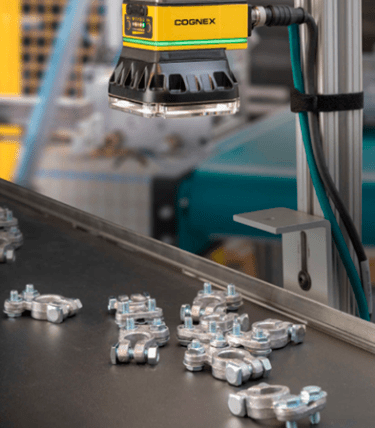
\includegraphics[width=0.85\textwidth]{vision_artificial.png}
     \end{center}
\end{column}
\end{columns}

\end{frame}

\section{Cámaras fotográficas}

\begin{frame}{Funcionamiento}
\begin{center}
    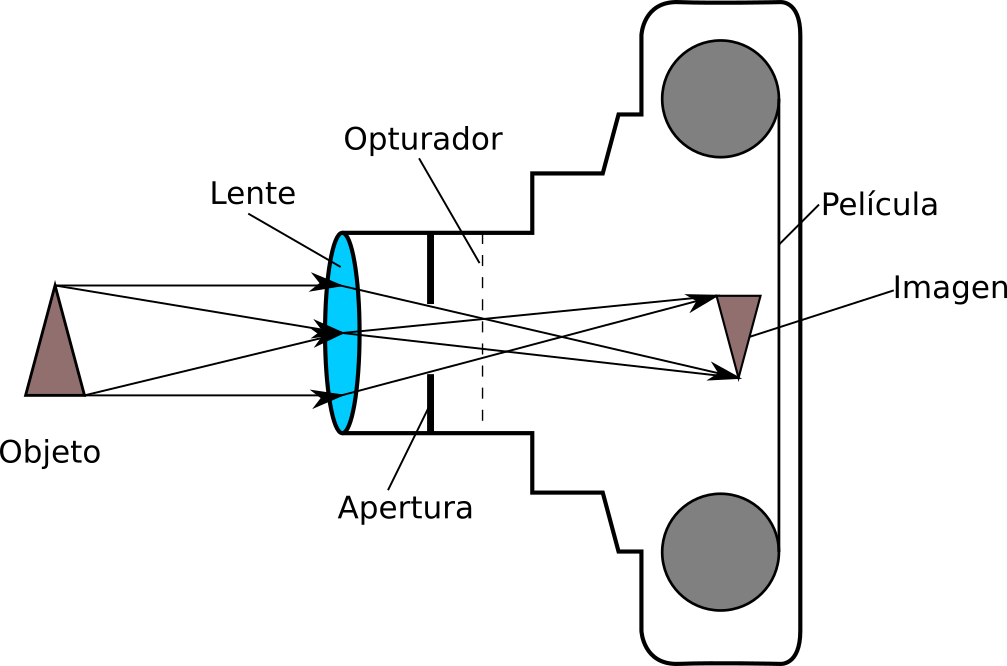
\includegraphics[width=0.8\textwidth]{cameraDiagram.png}
\end{center}
\end{frame}

\begin{frame}{Cámara analógica}
    % Funcionamiento
    % Componentes
    \begin{center}
        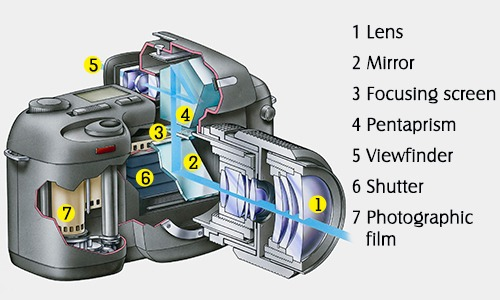
\includegraphics[width=0.8\textwidth]{analogDiagram.jpeg}
    \end{center}
\end{frame}

\begin{frame}{Cámara digital}
    % Funcionamiento
    % Componentes
    % http://edublog.amdsb.ca/myblogbenjamin394/2017/05/04/i-wonder-how-a-digital-camera-works/
    \begin{center}
        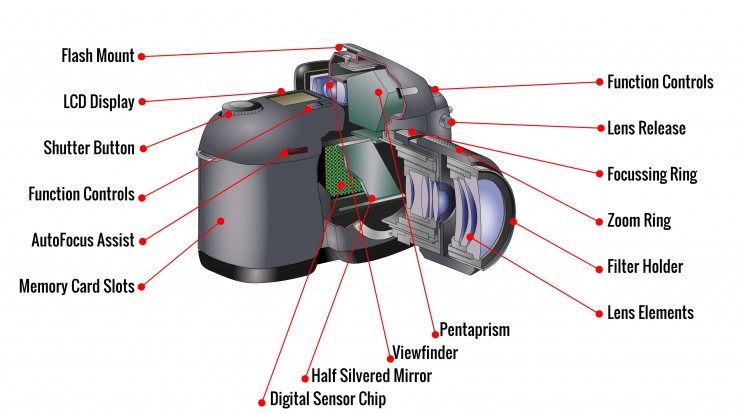
\includegraphics[width=\textwidth]{digitalDiagram.jpg}
    \end{center}
\end{frame}

\begin{frame}{Lentes}
    \begin{center}
        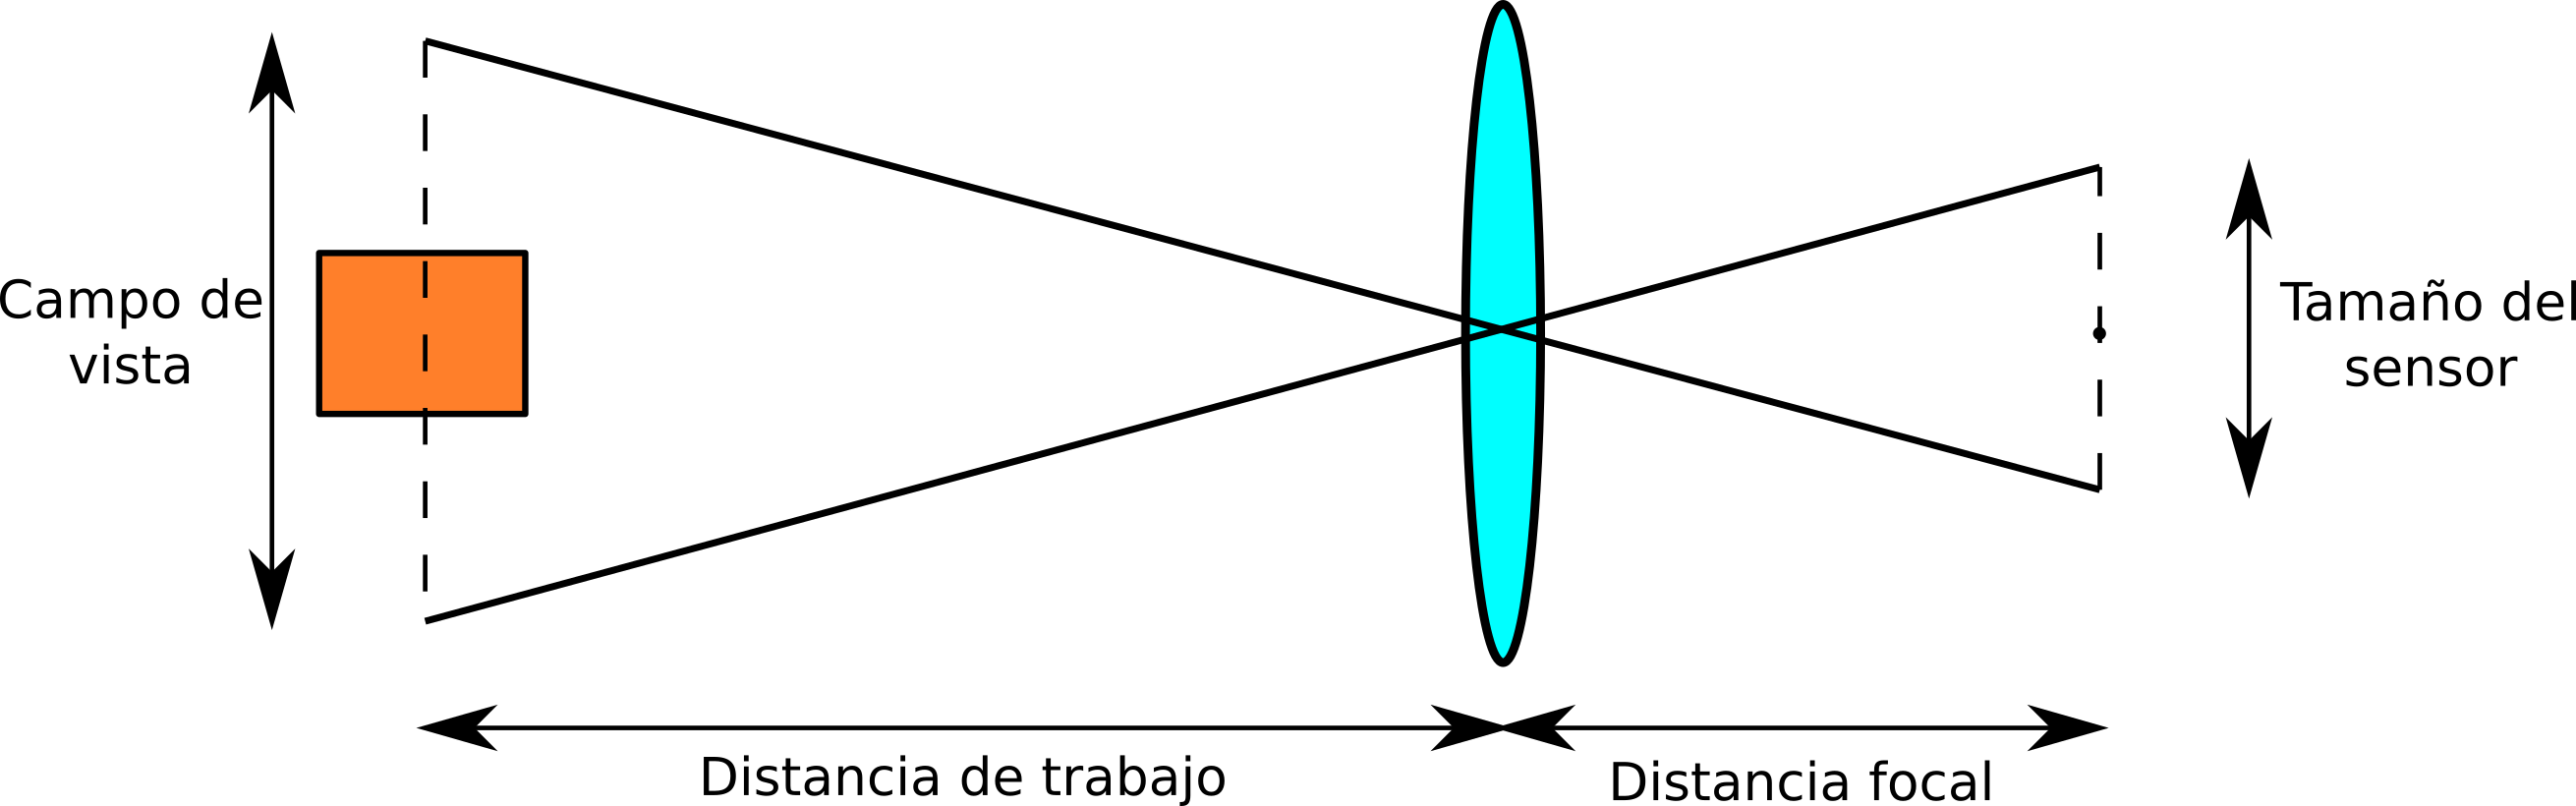
\includegraphics[width=\textwidth]{Lens.png}
    \end{center}
\end{frame}

\begin{frame}{Filtros}
    \begin{center}
        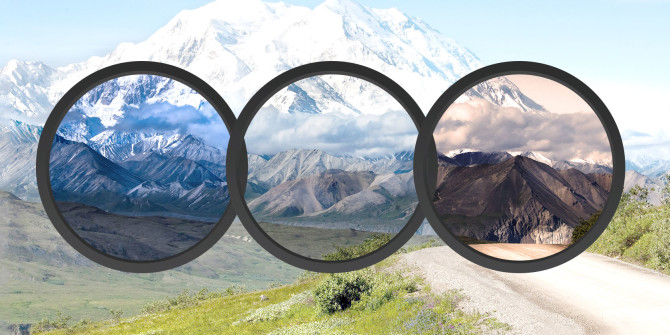
\includegraphics[width=0.8\textwidth]{filters.png}
    \end{center}
\end{frame}

\begin{frame}{Sensores}
\begin{center}
    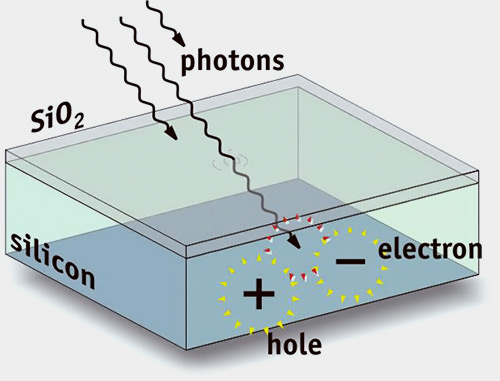
\includegraphics[width= 0.6\textwidth]{photons-hit-silicon.jpg}
\end{center}

    \begin{columns}
    \begin{column}{0.5\textwidth}
        CCD: Charged-Couple Device
    \end{column}
    \begin{column}{0.5\textwidth}
        CMOS: Complementary Metal Oxide Semi-conductor
    \end{column}
    \end{columns}
\end{frame}

\section{Cámara obscura}
\begin{frame}{Funcionamiento}
\begin{columns}
\begin{column}{0.5\textwidth}
     Se produce una imagen invertida de la escena observada.
\end{column}
\begin{column}{0.5\textwidth}  %%<--- here
    \begin{center}
     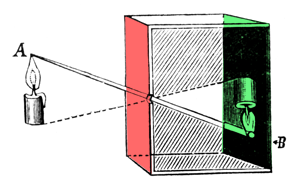
\includegraphics[width=\textwidth]{cameraobscura.png}
     \end{center}
\end{column}
\end{columns}
\end{frame}

\begin{frame}{Nitidez}
% Funcionamiento

\begin{center}
 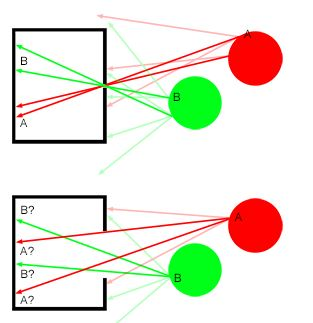
\includegraphics[width=5cm]{diametro.JPG}
\end{center}

\end{frame}

\begin{frame}{Ejemplos}
% Funcionamiento
\begin{center}
    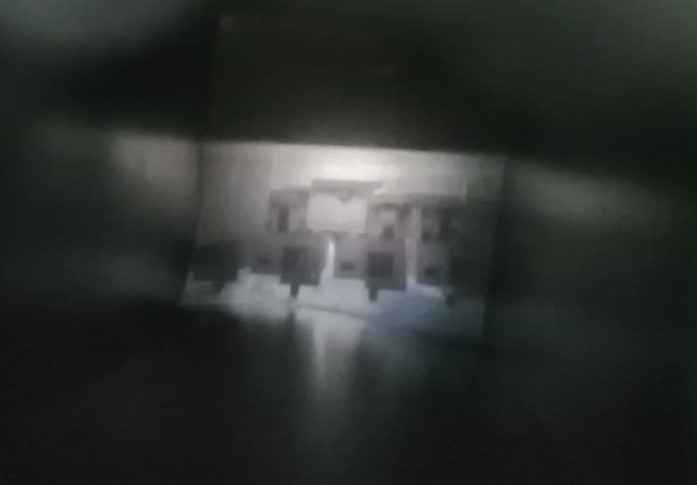
\includegraphics[width=0.8\textwidth]{camara_diy.jpeg}
\end{center}
\end{frame}

\begin{frame}{Catedral de Saltillo}
% Funcionamiento

\begin{center}
    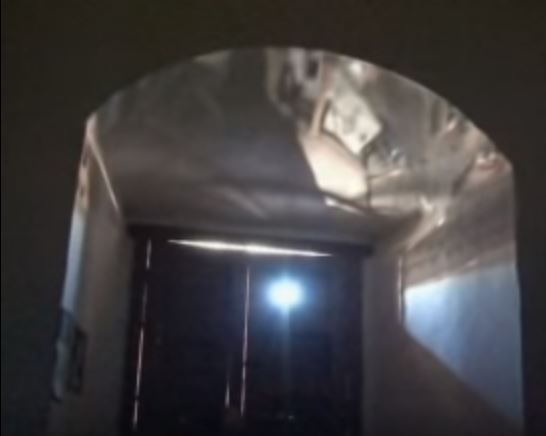
\includegraphics[width=0.8\textwidth]{catedral.JPG}
\end{center}
\end{frame}

%%%%%%%%%%%%%%%%%%%%%%%%%%%%%%%%%%%%

\section*{Referencias}
\begin{frame}{Referencias}
% \printbibliography{}
\begin{itemize}
    \item Nikon. Understanding Focal Length. Accesado 2020-02-03 en \hyperlink{www.nikonusa.com}{https://www.nikonusa.com/en/learn-and-explore/a/tips-and-techniques/understanding-focal-length.html}
    \item Adorama. A Beginner’s Guide to Camera Lens Filters. Accesado 2020-02-02 en \hyperlink{https://www.adorama.com/alc/a-beginners-guide-to-camera-lens-filters}{https://www.adorama.com/alc/a-beginners-guide-to-camera-lens-filters}
    \item Balihar, David. What is a pinhole camera? Accesado 2020-01-31 en \hyperlink{https://www.pinhole.cz/en/pinholecameras/whatis.html}{https://www.pinhole.cz/en/pinholecameras/whatis.html}
\end{itemize}

\end{frame}

\begin{frame}{Referencias}
    \begin{itemize}
        \item Teledyne DALSA. CCD vs CMOS. Accesado 2020-02-02 en \hyperlink{https://www.teledynedalsa.com/en/learn/knowledge-center/ccd-vs-cmos/}{https://www.teledynedalsa.com/en/learn/knowledge-center/ccd-vs-cmos/}
    \end{itemize}
\end{frame}

\end{document}
